\section{Negative results in full}
\label{app:negatives}

\paragraph{Novel-view synthesis (the null part of H4).} We initialize 3D Gaussian
Splatting~\cite{gsplat} from the predicted point map, optionally filtering or weighting points by each
uncertainty signal, optimize for a fixed budget, and render a held-out view. \Cref{fig:nvs} shows no
signal yields a meaningful PSNR advantage (all within $\sim 0.4$\,dB; random competitive). The
per-scene optimization (the Gaussians migrate and split until they fit the training views regardless
of where they started) absorbs the initialization differences, and NVS quality is dominated by
appearance/aleatoric factors rather than the epistemic geometry uncertainty \trustr\ captures. We
therefore report multi-view fusion (\Cref{sec:exp-fusion}) as the downstream utility. Reporting this
null prevents over-claiming and motivates the task where the signal is \emph{not} washed out.

\begin{figure}[h]
  \centering
  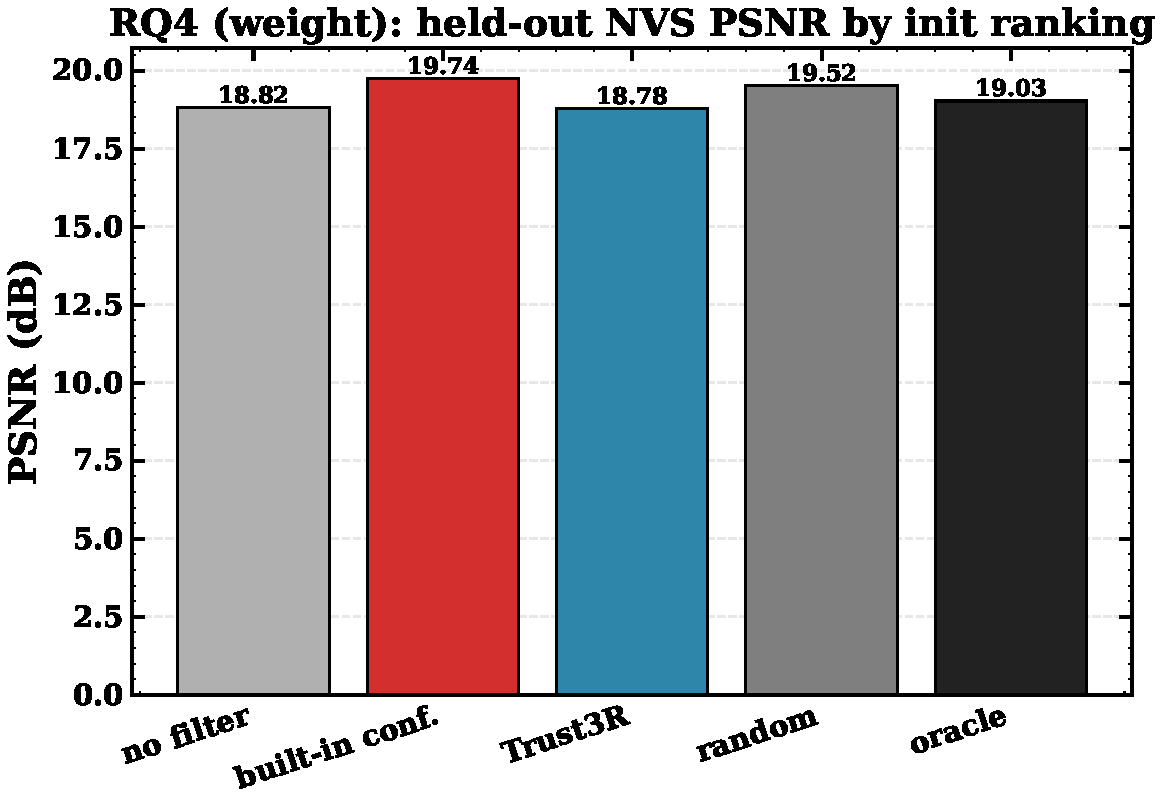
\includegraphics[width=0.85\linewidth]{rq4_psnr_weight_vggt.pdf}
  \caption{Uncertainty-weighted 3DGS-init NVS: held-out PSNR by ranking signal. No method separates;
  an honest null.}
  \label{fig:nvs}
\end{figure}

\begin{table}[h]
\centering\small
\adjustbox{max width=\columnwidth}{\input{tables/tab_downstream}}
\caption{Held-out NVS quality (weighted init) by ranking signal. No signal---including
\trustr---wins on PSNR\up/SSIM\up/LPIPS\dn; the gaps are within noise.}
\label{tab:downstream}
\end{table}

\paragraph{Falsified hypothesis (H3).} We hypothesized that view-permutation disagreement would be a
stronger signal for the reference-dependent \vggt\ than for the permutation-equivariant \pii. Relative
to each model's built-in confidence, the view-perm estimator reduces \ause\ by $19\%$ for \vggt\ but
$27\%$ for \pii---the opposite of the prediction. A plausible mechanism is that subset resampling perturbs the shared latent geometry
regardless of reference-dependence, and \pii's better-calibrated global point map retains more order
sensitivity. We report the characterization, not the original claim---the honest negative is itself
part of the contribution.
